\subsubsection{\stid{1.17} Open~MPI for Exascale (OMPI-X)}\label{subsubsect:openmpi}

%% {\itshape

%% 	\begin{enumerate}
%% 	\item Rename this file to your project WBS-projectname.tex, for example 2.3.3.01-XSDK4ECP.tex.
%% 	\item Complete this template for your project.  Limit your text to two pages, not counting citations.
%% 	\item Please avoid changing the content of main.tex.
%% 	\item Put any references in a .bib file with the same root name, for example 2.3.3.01-XSDK4ECP.bib.
%% 	\item Remember to include any image files you reference in your text.
%%     \item The files 2.3.3.01-XSDK4ECP.tex, 2.3.3.01-XSDK4ECP.bib and xSDK-diagram.jpeg are included as examples for your reference.  You can remove them from what you upload.
%% 	\end{enumerate}
%% }

\paragraph{Overview}
%% \textit{Provide an overview of your project.  You might find that the introductory text from your Fall 2017 Project Summary \url{https://confluence.exascaleproject.org/display/1ST/Fall+2017+ECP+ST+Project+Summaries} useful as a starting draft.}

The OMPI-X project ensures that the Message Passing Interface (MPI)
standard, and its specific implementation in Open~MPI meet the needs
of the ECP community in terms of performance, scalability, and
capabilities or features. MPI is the predominant interface for
inter-process communication in high-end computing.  Nearly all of the
ECP application (AD) projects (93\%~\cite{Bernholdt:2018:SMU-tr})
and the majority of software technology (ST) projects
(57\%~\cite{Bernholdt:2018:SMU-tr}) rely on it.
With the impending exascale era, the
pace of change and growing diversity of HPC architectures pose new
challenges that the MPI standard must address.  The OMPI-X project is
active in the MPI Forum standards organization, and works within it to
raise and resolve key issues facing ECP applications and libraries.

Open~MPI is an open source, community-based implementation of the MPI
standard that is used by a number of prominent
HPC vendors as the basis for their commercial MPI offerings.   The
OMPI-X team is comprised of active members of the Open~MPI community,
with an extensive history of contributions to this community.
The OMPI-X project focuses on prototyping
and demonstrating exascale-relevant proposals under consideration by
the MPI Forum, as well as improving the fundamental performance and
scalability of Open~MPI, particularly for exascale-relevant platforms
and job sizes.
MPI users will be able to take advantage of these
enhancements simply by linking against recent builds of the Open~MPI
library.

In addition to MPI and Open~MPI, the project also includes two other products,
which are less visible to the end user, but no less important.
PMIx (Process Management Interface for Exascale) provides facilities for
scalable application launch, process wire-up, resilience, and coordination between runtimes.
It originated as a spin-off from the Open~MPI community, but is now developing a
community of its own as adoption grows.  Through a recent (FY20) merger,
Qthreads (formerly WBS 2.3.1.15) is also part of the OMPI-X project.  Qthreads is a
user-level lightweight asynchronous thread library particularly focused on improving support for
multithreading in the context of network communications.  Both PMIx and Qthreads help the
OMPI-X project address key issues of performance and capability for exascale applications.


\paragraph{Key  Challenges}
%% \textit{Describe what is hard to do, why it is challenging.}
A number of aspects of ``exascale'' levels
of computing pose serious challenges to the ``tried and true'' message
passing model presented by MPI and its implementations, including Open~MPI.
%
Keeping pace with changes in HPC architecture is a major challenge.
Examples include massive node-level concurrency, driving the
growth of ``MPI+X'' programming approaches,
and the complex memory architectures, which make the placement of data
within memory more important. In the near-term, with GPUs dominating the exascale
environment, how code running on the GPUs interacts with MPI and inter-process
communications must also be addressed.  This will require both changes to the standard
and changes and improvements within implementations.
%
Performance and scalability become both more important and more
challenging as node counts increase
and memory per node trends downward.
%
Finally, as we identify solutions to these challenges that must be
``implemented'' within the MPI \emph{standard} rather than particular MPI libraries,
we must work within the much larger and broader MPI
community that may not always be attuned to the needs of computing at the largest scales.

\paragraph{Solution Strategy}
%% \textit{Describe your basic strategy for addressing the challenges.}
The OMPI-X project is working across a number of fronts to address
these challenges.

\emph{Runtime Interoperability for MPI+X and Beyond} MPI is
increasingly being used concurrently with other runtime environments.
This includes both ``MPI+X'' approaches, where X
is most often a threading model, such as OpenMP, as
well as the use of multiple inter-process runtimes within a single
application.  Concerns include awareness of other runtimes,
cooperative resource management capabilities, and ensuring that all
concurrently active runtimes make progress.  We are developing APIs and
demonstrating capabilities for interoperability in both MPI+X and
multiple inter-process runtime situations.

\emph{Extending the MPI Standard to Better Support Exascale
Architectures} The MPI community is considering for standardization a
number of ideas that
are particularly important to supporting
the architectural and system size characteristics anticipated for
exascale.  ``Partitioned communications'' (previously called ``Finepoints'')
deal with the growing use of threading for node-level concurrency, in
combination with MPI.  ``Sessions'' increases the flexibility of MPI
semantics in a number of areas, which in turn can open opportunities
for enhanced scalability, as well as easier support for
multi-component applications such as coupled multi-physics
simulations. Error management and recovery capabilities are key to
ensuring that applications can detect and respond effectively when errors,
inevitably, occur during execution.  We are helping to drive incorporation
of these and other ideas into the MPI standard by developing prototypes and
working with ECP teams and the broader community to demonstrate their
feasibility and value.

\emph{Open~MPI Scalability and Performance} As we push the scale of
both hardware and applications, we stress MPI implementations and
expose areas that need to be improved.
OMPI-X is targeting key components within Open~MPI, such as threading capabilities,
memory usage, remote memory access (RMA), tag matching, and other areas,
for improvements in both scalability and performance.

\emph{Supporting More Dynamic Execution Environments} We are
developing and implementing strategies to help MPI applications
better deal with topological process layout preferences
and contention in the network.

\emph{Resilience in MPI and Open~MPI} Concerns about system and
application resilience increase as either scales in size.  Our goal in
this area is to ensure that MPI, Open~MPI, and PMIx provide not only
support for simplified
recovery for the widely used checkpoint/restart fault tolerance strategy, but also the building
blocks to support more general error management and recovery by applications (the evolution of the User-Level
Fault Mitigation concept). We work within the MPI Forum, implement,
and train users on resilience strategies.

\emph{MPI Tools Interfaces}  Several interfaces within the
MPI standard are primarily used to support performance and
correctness tools.
The MPI Forum is in the process
of making significant revisions and extensions to these interfaces.
We will track the discussions in the Forum and provide prototype
implementations within Open~MPI to facilitate evaluation and provide
feedback.
We will work with the
ECP community, including tool developers, to make additional data
available through the MPI\_T interface.

\emph{Quality Assurance for Open~MPI}  We are enhancing the
Open~MPI testing infrastructure, adding tests to reflect ECP
requirements, and instantiating routine testing on systems of
importance to ECP, both for correctness and performance.

\begin{figure}
\centering
\begin{minipage}[c]{0.20\textwidth}
\captionsetup{width=\textwidth,font=small,labelfont=bf} %% Need to override default width
\caption{ReInit reduces the time for applications to recover from faults using checkpoints.}
\label{fig:partitioned-communications}
\end{minipage}
\qquad
\begin{minipage}[c]{0.20\textwidth}
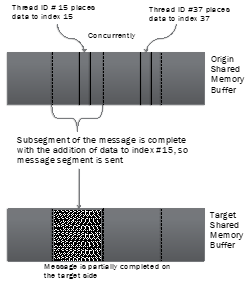
\includegraphics[width=\textwidth]{projects/2.3.1-PMR/2.3.1.17-OMPI-X/partitioned-communications-partial-sends.png}
\end{minipage}
\qquad
\begin{minipage}[c]{0.33\textwidth}
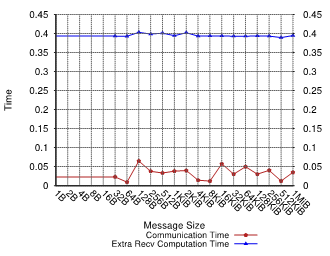
\includegraphics[width=\textwidth]{projects/2.3.1-PMR/2.3.1.17-OMPI-X/partitioned-communications-early-receive.png}
\end{minipage}
\end{figure}

\begin{wrapfigure}{r}{0.40\textwidth}
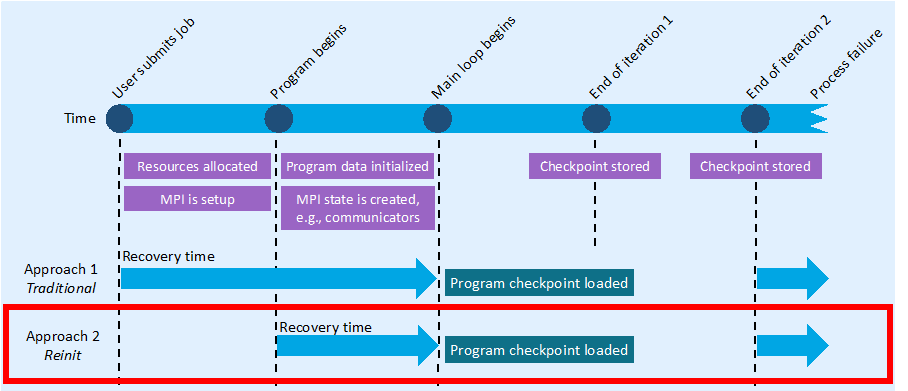
\includegraphics[width=0.40\textwidth]{projects/2.3.1-PMR/2.3.1.17-OMPI-X/reinit.png}
\caption{ReInit reduces application recovery time.}
\label{fig:reinit}
\end{wrapfigure}

\paragraph{Recent Progress}
%% \textit{Describe what you have done recently.  It would be good to
%% have some kind of figure or diagram in this section.}
There has been a great deal of activity within the MPI standards community recently
as they work to finalize the feature set for MPI 4.0 by December 2019 and
formal adoption by November 2020.  A number of error management and recovery features
championed by the OMPI-X team have already been formally voted into 4.0.  The Sessions proposal,
also driven significantly by OMPI-X is considered a mandatory feature
for 4.0.  And it is considered extremely likely that Partitioned
Communications (Figure~\ref{fig:partitioned-communications}), led by
OMPI-X, will also make version 4.0. 
In the longer-term discussions, OMPI-X is also championing the
``ReInit'' proposal for simplified checkpoint/restart application
recovery (Figure~\ref{fig:reinit}) and is actively engaged on other topics relevant to
exascale, including MPI\_T events, enhanced hardware topologies, thread safety enhancements, half-precision datatypes, and a replacement for the PMPI interface.  ECP (mini-) applications which have been used in demonstrating various features and capabilities include: AMG, CoMD, LULESH, miniFE, miniMD, NWChemEx, and SimpleMOC.

Motivated largely by support for the Partitioned Communications proposal and other situations where high network concurrency is required, a general user-level threading abstraction has been developed to support both the Qthreads and BOLT/Argobots threading libraries within either the Open~MPI or MPICH libraries.  This work, carried out in collaboration with the MPICH and Argobots ECP teams (WBS 2.3.1.07 and 2.3.5.05) is in the process of being integrated into the two MPI implementations.

To provide better long-term support for resilience, a number of fault detection and coordination features have been refactored out of Open~MPI and moved into the PMIx implementation, where they can benefit to a larger community of programming models, including all other runtimes and tools that use PMIx.  The OMPI-X team has also played an active role in helping the PMIx community grow and formalize its processes within the last year.  This includes separating the standard from the reference implementation, and establishing and documenting governance procedures for both.  This will allow the PMIx community to better deal with the strong uptick in interest and actual and potential PMIx clients recently.

Two areas of progress on supporting exacale-relevant architectures include complex memory and topology/congestion awareness within the MPI library. In collaboration with the ECP SICM project (WBS 2.3.1.16), we are integrating support for complex memory architectures into Open~MPI.  This will enable controlled placement of data objects within different memory spaces according to affinity and/or performance characteristics.  The ability to detect and adapt to network topology and traffic patterns is also a valuable capability to facilitate application performance which has been prototyped within Open~MPI.

In support of better ``MPI+X'' interoperability, we have redesigned the internal Open~MPI infrastructure to minimize contention on the execution path of independent MPI operations and optimize the handling of MPI requests, drastically improving the communication, point-to-point, RMA and collective, performance of Open~MPI in threaded contexts. In addition the progress engine has been reimplemented to maximize the opportunity for computation/communication overlap, and provide a guarantee for asynchronous progress when possible. Using these capabilities we also demonstrated fined-grained control of thread and process placement in the context of OpenMP and Open~MPI, in collaboration with the SOLLVE ECP project (WBS 2.3.2.11). Such a capability is crucial to the ability of MPI+X applications to effectively utilize current and future ``fat'' node architectures (with extensive compute capabilities), but can be hard or impossible to achieve unless the two runtimes are made aware of each other and (minimally) cooperate on resource management.
%
Because poor performance with threading is one of the most common
complaints against (any) MPI implementations, a great deal of our
recent effort has been devoted to improving this in various ways
within Open~MPI.  We have redesigned point-to-point and remote
memory access request management, and redesigned the progress engine
for better performance with threads (Figure~\ref{fig:threading-performance}).
Moreover, the Partitioned Communications proposal, mentioned above also targets threaded execution by increasing opportunities for fine-grained overlap of computation with communication and reduced locking.  We have also improved the message matching implementation so support faster message rates and high thread counts.

\begin{figure}
\centering
\begin{minipage}[c]{0.2\textwidth}
\captionsetup{width=\textwidth,font=small,labelfont=bf} %% Need to override default width
\caption{Performance of point-to-point (left) and remote memory access
(right) communication with threading.} 
\label{fig:threading-performance}
\end{minipage}
\qquad
\begin{minipage}[c]{0.2\textwidth}
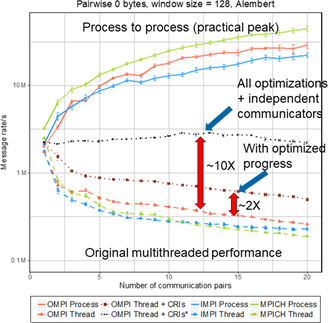
\includegraphics[width=\textwidth]{projects/2.3.1-PMR/2.3.1.17-OMPI-X/p2p-threading-performance.png}
\end{minipage}
\qquad
\begin{minipage}[c]{0.5\textwidth}
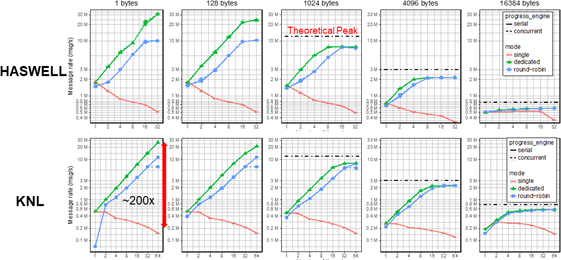
\includegraphics[width=\textwidth]{projects/2.3.1-PMR/2.3.1.17-OMPI-X/rma-threading-performance.png}
\end{minipage}
\end{figure}

Finally, we continue to extend the testing infrastructure for Open~MPI and related products, increasing the platforms on which testing is implemented, and expanding the repertoire of tests.  We have enhanced the MTT tool used for testing of Open~MPI itself, and supplemented it with a new tool aimed at testing of application kernels and performance testing.  We have deployed testing capabilities on Summit, and are also testing on Cori.


\paragraph{Next Steps}
%% \textit{Describe what you are working on next.}
In FY20 and beyond, we plan to continue working across the multiple fronts described above.  Finalizing version 4.0 of the MPI standard will be an important part of our work in FY20, as part of the larger community.  Since the first exascale systems have now been announced, we can also start incorporating activities targeted to those specific systems into our work as well.  Both the Argonne and Oak Ridge systems will utilize Cray's SlingShot network, which is currently under active development.  NERSC's Perlmutter system will include SlingShot version 10, while Aurora and Frontier will use version 11.
